\quad U ovom poglavlju obrađujemo implementacijske detalje sustava baziranog na CGP-u korištenog u radu i promjene učinjenje u verziji korištene igre.
\section{Osnovne informacije}
\quadČitava implementacija napravljena je u programskom jeziku Java (verzija 19.0.1). Sustav baziran na CGP-u napravljen je u obliku klase imena \textit{CGP} i ukomponiran je u paket igre. Sustav stvara i koristi dodatne dvije txt datoteke u kojima se drže rezultati treniranja (\textit{scores.txt}) i zadnja populacija programa s kojom je sustav radio (\textit{population.txt}). Programi se zapisuju u obliku niza brojeva po uzoru na zapis opisan u poglavlju 4 uz parametar l=$ n_{c} $. Modifikacije verzije igre napravljene su u postojećim klasama.
\par 
Sustav za treniranje programa koncipiran je poput podržanog učenja s brojem generacija kao uvjetom zaustavljanja. Program nakon kraja igre dobiva rezultat (eng. score) koji služi kao dio dobrote programa. Svaki program ima unaprijed zadan broj ponavljanja igranja igre. Ponavljanja su uvedena zbog elemenata nasumičnosti igre i njima se pokušava smanjiti utjecaj elemenata na ocjenu uspješnosti programa. Konačna ocjena uspješnosti programa bit će dana nakon zadnjeg ponavljanja i bit će srednja vrijednost svih dobivenih rezultata.
\par
\section{Programi}
\quad Implementacijska ideja kreće od koncepta programa. Koje podatke prenijeti programu? Kako bi program trebao signalizirati svoju odluku o smjeru pomicanja elementa?
\par
Radi olakšanja rada, programi su tijekom treniranja sadržani u objektima klase \textit{Individula}. Klasa \textit{Individual} sadržava: originalni zapis programa, program podijeljen u čvorove, rezultate dobivene igranjem igre, srednji rezultat igara, popis aktivnih čvorova, širinu mreže, dužinu mreže, broj čvorova, broj ulaza, broj izlaza i generacija nastanka. Svi podaci, osim rezultata, dani su pri samoj inicijalizaciji objekta.
\par 
Stanje ploče prenosi se programu u svakom koraku igre. S obzirom na to da ploča sadrži 16 polja, program ima 16 ulaza u mrežu. Stanje ploče prenosi se u obliku liste brojeva gdje se slijedno zapisuju polja ploče od gornje lijeve pozicije do donje desne. Brojevima od 0 do 12 zapisuje se sadržaj polja. 0 se koristi kao oznaka da je polje prazno, a ostali brojevi predstavljaju vrijednosti koje se mogu pojaviti u polju i možemo gledati na njih kao na eksponente na broj 2. U primjeru na slici 8.1 prva lista prikazuje početno stanje ploče. U početnom stanju vrijednost 2 pojavljuje se na dva mjesta; treći red i četvrti stupac, četvrti red i treći stupac.
 \begin{figure}[h]
	\centering
	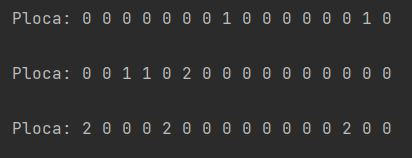
\includegraphics[width=0.6\linewidth]{imp_4}
	\caption{Stanje ploče tijekom tri poteza}
\end{figure}

\par
Završetkom obrade podataka u mreži, konačni rezultati dovode se na četiri izlaza. Svaki izlaz signalizira pokret u određenom smjeru (gore, desno, dolje, lijevo). Izlaz s najvećom vrijednošću predstavlja odluku programa.
\par
Stanje ploče nije bilo praćeno u igri te je uvedeno tijekom ovog rada u klasu \textit{Spavner}. Uvođenjem modifikacija u klasu, \textit{Spavner} pohranjuje i obnavlja stanje ploče nakon svakog poteza. Ustanovi li se da je ploča puna i da više nema mjesta za novi element, ploča se čisti, a sprema se lista nula koja signalizira da je igra završila. Završetkom igre programu se šalje rezultat partije. Nakon takvog kraja igre ploča se ponovo postavlja u početno stanje spremno za novu igru.
\
\par 
\section{Pokretanje treniranja}
\quad Sustav za treniranje programa može se pokrenuti na dva načina. Nakon pokretanja igre, pritiskom na tipku \textit{0} pokreće se metoda sa slike 8.2 koja briše zapis prošle generacije s kojom je sustav radio iz \textit{population.txt}, ako postoji; stvara se nova početna generacija i započinje treniranje.
\begin{figure}[h]
	\centering
	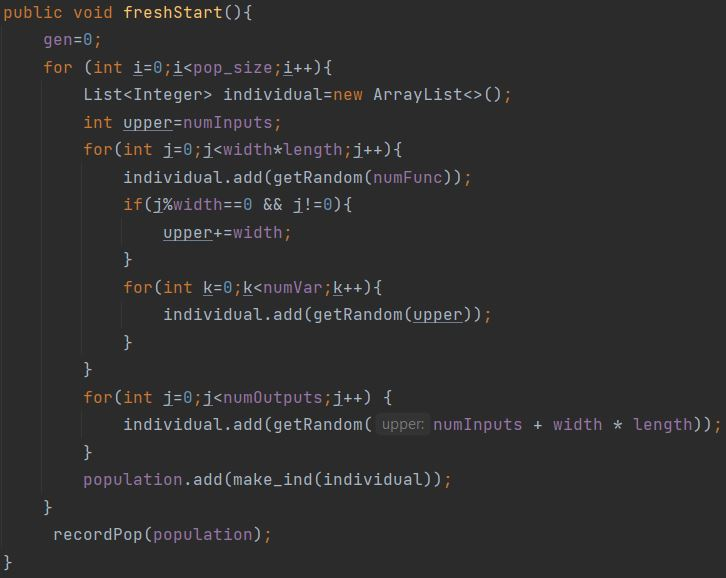
\includegraphics[width=0.6\linewidth]{fresh_start}
	\caption{Metoda inicijalizacije nove početne populacije aktivirana pritiskom na tipku \textit{0}}
\end{figure}
\par Pritiskom na tipku \textit{4} nastavljamo treniranje populacije zapisane u \textit{population.txt}. Populacija se zapisuje u \textit{population.txt} prilikom inicijalizacije sasvim nove populacije ili nakon generiranja nove generacije. Dodatni parametri koji se šalju u zapis osim programa su širina i duljina mreže te trenutna generacija. Slika 8.3 prikazuje metodu koja zapisuje populaciju.
\begin{figure}[h]
	\centering
	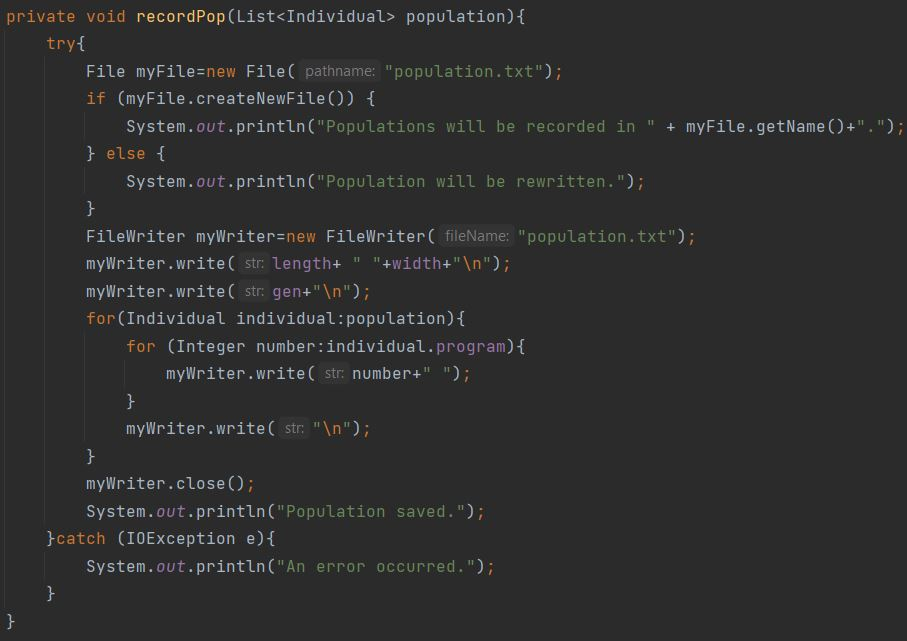
\includegraphics[width=0.6\linewidth]{recordPop}
	\caption{Metoda spremanja populacije u \textit{population.txt}}
\end{figure}\newline
\par
 Početni parametri programa i sustava (broj redova, broj stupaca, veličina populacije, broj ponavljanja) zadaju se u \textit{KeyInput} klasi kod inicijalizacije objekta klase CGP. Dodatni parametri poput generacijske granice, mogućih funkcija i broja mutacija mogu se podesiti unutar klase \textit{CGP}, s napomenom kako promjena mogućih funkcija zahtijeva više promjena implementacije i veći oprez.
\par
Zadnji korak u pokretanju treniranja je stvaranje dretve koja će provoditi treniranje. Ovime glavnu dretvu vraćamo održavanju igre i grafičkog sučelja te postižemo paralelan rad.
\section{Igranje igre}
\quad Dretva zadužena za treniranje kontinuirano dohvaća stanje ploče. Ako na ploči postoje elementi, stanje ploče se prosljeđuje metodi \textit{predict} (Slika 8.4) koja izvodi trenutni program na način koji je opisan u potpoglavlju 4.6. Metoda vraća broj izlaza s najvećom vrijednosti. Odluka o pomicanju elemenata donosi se na osnovu dobivenog broja. 
\par
Ako na ploči nema elemenata to znači kako je igra završila. Spremamo rezultate i pozivamo metodu \textit{keep\_count} (slika 8.5) koja prati koji program se izvodi, koliko puta se izveo i nalazimo li se na prijelazu u novu generaciju.
\begin{figure}[h]
	\centering
	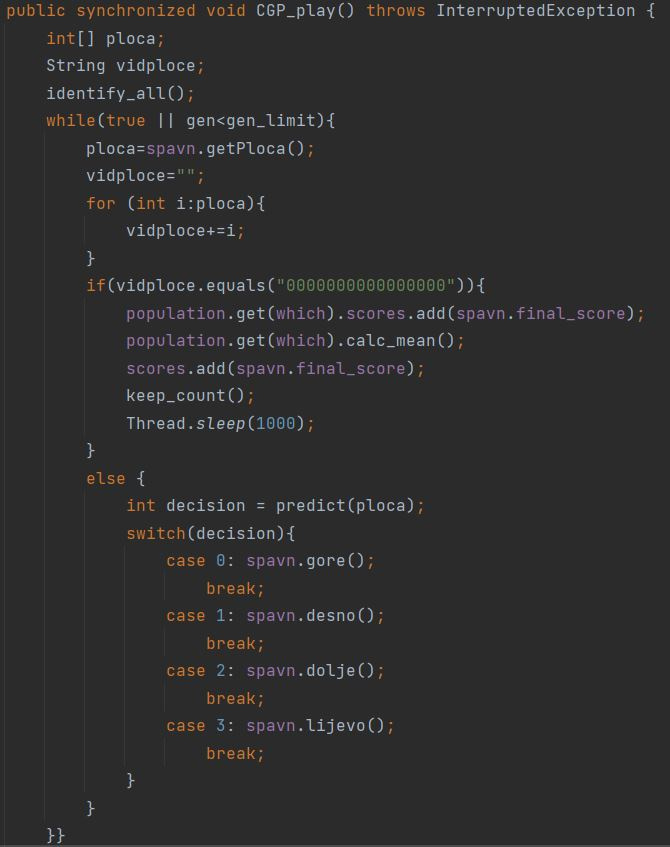
\includegraphics[width=0.6\linewidth]{cgpPlay}
	\caption{Metoda kontinuiranog provođenja igranja igre}
\end{figure}\newline
\begin{figure}[h]
	\centering
	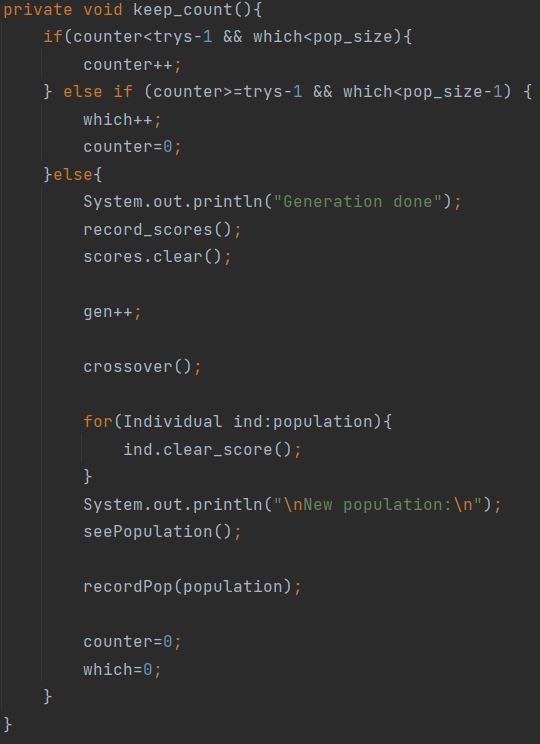
\includegraphics[width=0.6\linewidth]{keep_count}
	\caption{Metoda praćenja programa i generacija}
\end{figure}\newline
\section{Selekcija i križanje}
\quad Metoda \textit{keep\_count} prepoznaje kraj generacije, zapisuje vrijeme zapisa, parametre sustava, rezultate svakog programa i pokreće operaciju selekcije i križanja. Selekcija je implementirano kao turnir s nasumičnim izborom programa. Broj programa koje odabiremo je varijabilan, ali je uvijek višekratnik broja četiri. Razlog tome je taj da odabiremo dva para po dva programa. Programe u paru međusobno uspoređujemo. Programi koji su unutar para bili bolji križaju se, a gori će biti zamijenjeni djecom boljih. Bolji programi i programi koji nisu sudjelovali u turnirima prelaze u novu generaciju. Ovime se donekle ostvaruje elitizam jer najbolji programi na jedan ili na drugi način prelaze u sljedeću generaciju.
\par 
Implementirane su dvije metode križanja. Prva metoda se može smatrati destruktivnom i najmanje je korištena u testovima. Implementirana je za mreže sa širinom većom od jedan. Metoda stvara dvoje djece tako da svaki čvor djeteta ima 50\% šanse doći od jednog ili od drugog roditelja. Destruktivnost proizlazi iz činjenice da se na ovaj način genima jednog roditelja remete dijelovi genotipa drugog roditelja koji su ga činili uspješnim. (Slike 8.6 (a) i (b))
\begin{figure}[h]
	\centering
	\begin{subfigure}{0.4\textwidth}
		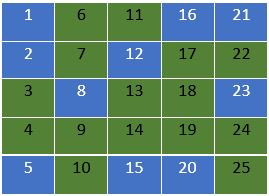
\includegraphics[width=0.9\linewidth]{my_cgp_cross_1} 
		\caption{Prvo dijete}
	\end{subfigure}
	\begin{subfigure}{0.4\textwidth}
		{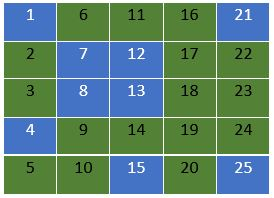
\includegraphics[width=0.9\linewidth]{my_cgp_cross_2}}
		\caption{Drugo dijete}
	\end{subfigure}
	\caption{Primjer rezultata prve metode križanja}
\end{figure}
\par
Druga metoda implementirana je za mreže širine 1 i zasnovana je na križanju s jednom točkom prijeloma. Kopije dva roditelja se prepolove u odabranom čvoru, a zatim se svaki dio spoji s dijelom drugog programa. 
\begin{figure}[h]
	\centering
	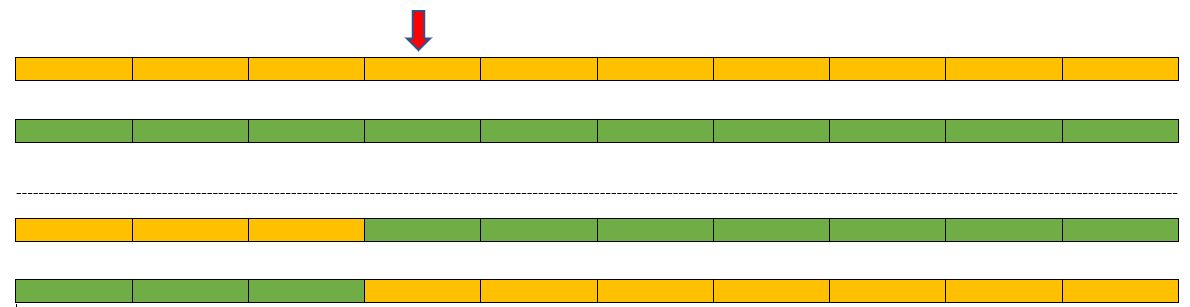
\includegraphics[width=0.6\linewidth]{crossover_point}
	\caption{Križanje s jednom točkom prijeloma}
\end{figure}

\section{Mutacija}
\quad Implementirane su dvije vrste mutacija, mutacija postotka i single mutacija, ali u testovima je korištena samo single mutacija kako bi se smanjila mogućnost potencijalno prevelike promjene fenotipa. Implementacija (Slika 8.8) dodatno omogućuje odabir broja uzastopnih single mutacija djeteta u svrhu proširenja područja testiranja. Single mutacija olakšana je činjenicom da objekti klase \textit{Individual} već sadrže popis aktivnih gena pa stvaramo listu gena za mutaciju dok ne odaberemo gen s popisa aktivnih gena. Jednom kad se aktivni gen odabere, prestajemo tražiti gene za mutaciju, a odabrane gene izmijenimo.
\par 
 Mutacijom završavamo naš proces stvaranja djece. Novonastala djeca pridružuju se već postojećoj populaciji dolaskom na mjesto programa koji su se iskazali slabijima u procesu selekcije. Time započinjemo novu generaciju, a podaci o novoj populaciji spremaju se u \textit{population.txt}
 
\begin{figure}[h]
	\centering
	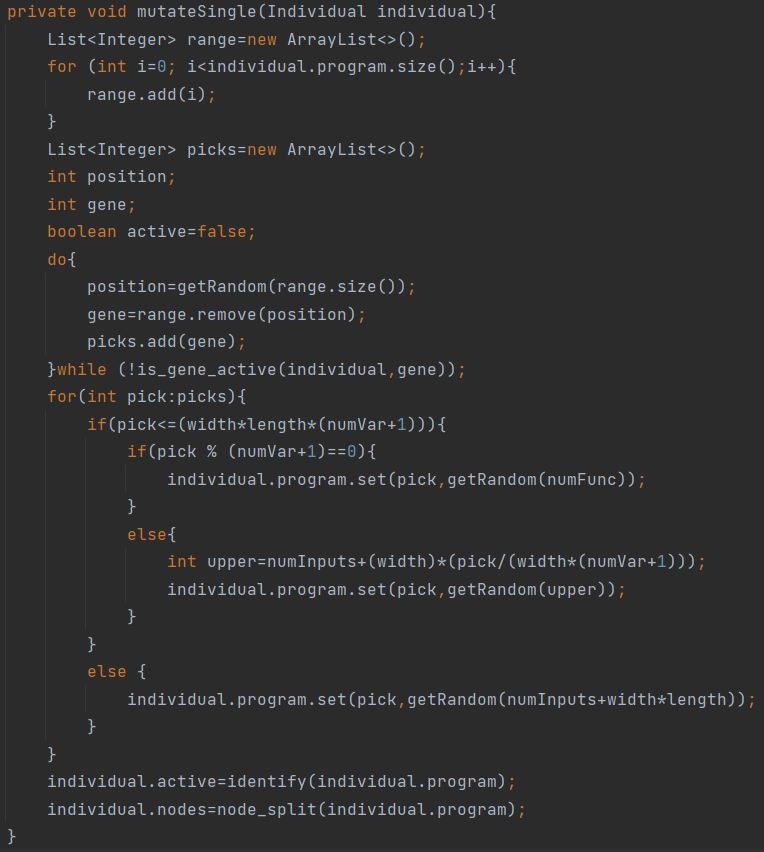
\includegraphics[width=0.6\linewidth]{my_cgp_mutation}
	\caption{Metoda Single mutacije}
\end{figure}

\newpage
\verb| |